\documentclass{standalone}
\usepackage{tikz}
\usetikzlibrary{patterns, positioning}

\begin{document}
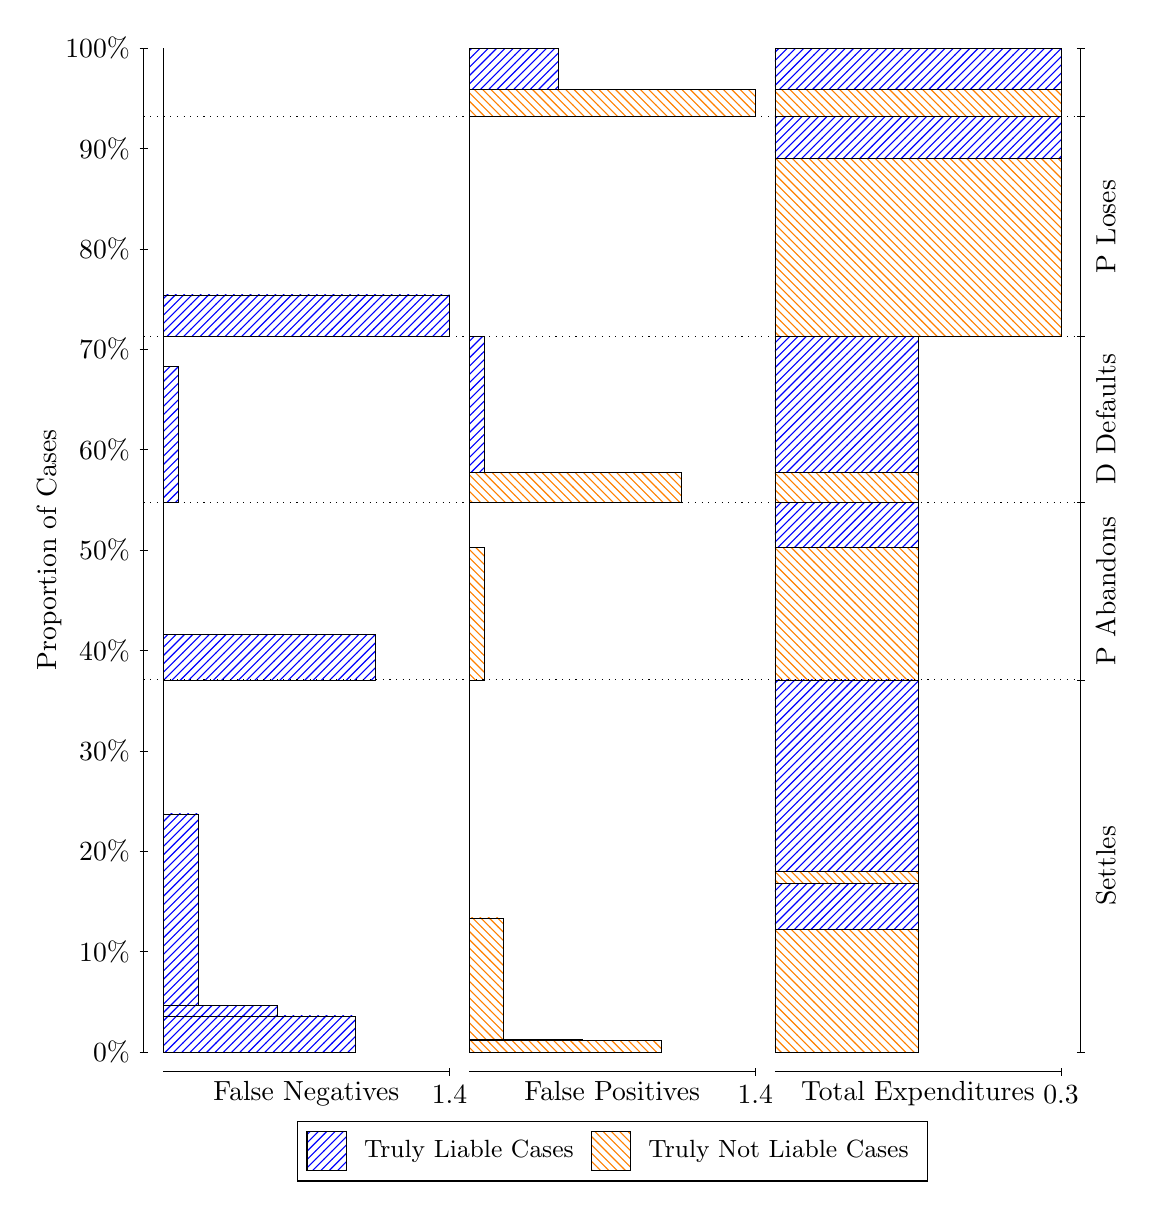
\begin{tikzpicture}
\draw[black, very thin] (1.5,1.75) -- (1.5,14.5);
\node[rotate=90, anchor=center] at (0.3, 8.125) {Proportion of Cases};
\draw[black, very thin] (1.45,1.75) -- (1.55,1.75);
\node[anchor=east] at (1.45, 1.75) {0\%};
\draw[black, very thin] (1.45,3.025) -- (1.55,3.025);
\node[anchor=east] at (1.45, 3.025) {10\%};
\draw[black, very thin] (1.45,4.3) -- (1.55,4.3);
\node[anchor=east] at (1.45, 4.3) {20\%};
\draw[black, very thin] (1.45,5.575) -- (1.55,5.575);
\node[anchor=east] at (1.45, 5.575) {30\%};
\draw[black, very thin] (1.45,6.85) -- (1.55,6.85);
\node[anchor=east] at (1.45, 6.85) {40\%};
\draw[black, very thin] (1.45,8.125) -- (1.55,8.125);
\node[anchor=east] at (1.45, 8.125) {50\%};
\draw[black, very thin] (1.45,9.4) -- (1.55,9.4);
\node[anchor=east] at (1.45, 9.4) {60\%};
\draw[black, very thin] (1.45,10.675) -- (1.55,10.675);
\node[anchor=east] at (1.45, 10.675) {70\%};
\draw[black, very thin] (1.45,11.95) -- (1.55,11.95);
\node[anchor=east] at (1.45, 11.95) {80\%};
\draw[black, very thin] (1.45,13.225) -- (1.55,13.225);
\node[anchor=east] at (1.45, 13.225) {90\%};
\draw[black, very thin] (1.45,14.5) -- (1.55,14.5);
\node[anchor=east] at (1.45, 14.5) {100\%};

\draw[black, very thin] (13.4,1.75) -- (13.4,14.5);
\draw[black, very thin] (13.35,1.75) -- (13.45,1.75);
\node[anchor=west] at (13.35, 1.75) {};
\draw[black, very thin] (13.35,6.4764) -- (13.45,6.4764);
\node[anchor=west] at (13.35, 6.4764) {};
\draw[black, very thin] (13.35,8.73) -- (13.45,8.73);
\node[anchor=west] at (13.35, 8.73) {};
\draw[black, very thin] (13.35,10.84) -- (13.45,10.84);
\node[anchor=west] at (13.35, 10.84) {};
\draw[black, very thin] (13.35,13.627) -- (13.45,13.627);
\node[anchor=west] at (13.35, 13.627) {};
\draw[black, very thin] (13.35,14.5) -- (13.45,14.5);
\node[anchor=west] at (13.35, 14.5) {};

\draw[black, very thin, pattern color=blue, pattern=north east lines] (1.75,1.75) rectangle (4.1931,2.2081);
\draw[black, very thin, pattern color=blue, pattern=north east lines] (1.75,2.2081) rectangle (3.1908,2.338);
\draw[black, very thin, pattern color=blue, pattern=north east lines] (1.75,2.338) rectangle (2.9402,2.3392);
\draw[black, very thin, pattern color=blue, pattern=north east lines] (1.75,2.3392) rectangle (2.6897,2.3404);
\draw[black, very thin, pattern color=blue, pattern=north east lines] (1.75,2.3404) rectangle (2.4391,2.3418);
\draw[black, very thin, pattern color=blue, pattern=north east lines] (1.75,2.3418) rectangle (2.1885,4.7725);
\draw[black, very thin, pattern color=orange, pattern=north west lines] (1.75,4.7725) rectangle (1.75,6.4764);
\draw[black, very thin, pattern color=blue, pattern=north east lines] (1.75,6.4764) rectangle (4.4437,7.0496);
\draw[black, very thin, pattern color=orange, pattern=north west lines] (1.75,7.0496) rectangle (1.75,8.73);
\draw[black, very thin, pattern color=blue, pattern=north east lines] (1.75,8.73) rectangle (1.9379,10.461);
\draw[black, very thin, pattern color=orange, pattern=north west lines] (1.75,10.461) rectangle (1.75,10.84);
\draw[black, very thin, pattern color=blue, pattern=north east lines] (1.75,10.84) rectangle (5.3833,11.365);
\draw[black, very thin, pattern color=orange, pattern=north west lines] (1.75,11.365) rectangle (1.75,13.627);
\draw[black, very thin, pattern color=orange, pattern=north west lines] (1.75,13.627) rectangle (1.75,13.978);
\draw[black, very thin, pattern color=blue, pattern=north east lines] (1.75,13.978) rectangle (1.75,14.5);
\draw[black, very thin, pattern color=orange, pattern=north west lines] (5.6333,1.75) rectangle (8.0764,1.8993);
\draw[black, very thin, pattern color=orange, pattern=north west lines] (5.6333,1.8993) rectangle (7.8259,1.8994);
\draw[black, very thin, pattern color=orange, pattern=north west lines] (5.6333,1.8994) rectangle (7.5753,1.8995);
\draw[black, very thin, pattern color=orange, pattern=north west lines] (5.6333,1.8995) rectangle (7.3247,1.8996);
\draw[black, very thin, pattern color=orange, pattern=north west lines] (5.6333,1.8996) rectangle (7.0741,1.9097);
\draw[black, very thin, pattern color=orange, pattern=north west lines] (5.6333,1.9097) rectangle (6.0718,3.4538);
\draw[black, very thin, pattern color=blue, pattern=north east lines] (5.6333,3.4538) rectangle (5.6333,6.4764);
\draw[black, very thin, pattern color=orange, pattern=north west lines] (5.6333,6.4764) rectangle (5.8213,8.1567);
\draw[black, very thin, pattern color=blue, pattern=north east lines] (5.6333,8.1567) rectangle (5.6333,8.73);
\draw[black, very thin, pattern color=orange, pattern=north west lines] (5.6333,8.73) rectangle (8.327,9.1082);
\draw[black, very thin, pattern color=blue, pattern=north east lines] (5.6333,9.1082) rectangle (5.8213,10.84);
\draw[black, very thin, pattern color=orange, pattern=north west lines] (5.6333,10.84) rectangle (5.6333,13.101);
\draw[black, very thin, pattern color=blue, pattern=north east lines] (5.6333,13.101) rectangle (5.6333,13.627);
\draw[black, very thin, pattern color=orange, pattern=north west lines] (5.6333,13.627) rectangle (9.2667,13.978);
\draw[black, very thin, pattern color=blue, pattern=north east lines] (5.6333,13.978) rectangle (6.7609,14.5);
\draw[black, very thin, pattern color=orange, pattern=north west lines] (9.5167,1.75) rectangle (11.333,3.3042);
\draw[black, very thin, pattern color=blue, pattern=north east lines] (9.5167,3.3042) rectangle (11.333,3.8922);
\draw[black, very thin, pattern color=orange, pattern=north west lines] (9.5167,3.8922) rectangle (11.333,4.0418);
\draw[black, very thin, pattern color=blue, pattern=north east lines] (9.5167,4.0418) rectangle (11.333,6.4764);
\draw[black, very thin, pattern color=orange, pattern=north west lines] (9.5167,6.4764) rectangle (11.333,8.1567);
\draw[black, very thin, pattern color=blue, pattern=north east lines] (9.5167,8.1567) rectangle (11.333,8.73);
\draw[black, very thin, pattern color=orange, pattern=north west lines] (9.5167,8.73) rectangle (11.333,9.1082);
\draw[black, very thin, pattern color=blue, pattern=north east lines] (9.5167,9.1082) rectangle (11.333,10.84);
\draw[black, very thin, pattern color=orange, pattern=north west lines] (9.5167,10.84) rectangle (13.15,13.101);
\draw[black, very thin, pattern color=blue, pattern=north east lines] (9.5167,13.101) rectangle (13.15,13.627);
\draw[black, very thin, pattern color=orange, pattern=north west lines] (9.5167,13.627) rectangle (13.15,13.978);
\draw[black, very thin, pattern color=blue, pattern=north east lines] (9.5167,13.978) rectangle (13.15,14.5);
\draw[black, dotted] (1.5,6.4764) -- (13.4,6.4764);
\draw[black, dotted] (1.5,8.73) -- (13.4,8.73);
\draw[black, dotted] (1.5,10.84) -- (13.4,10.84);
\draw[black, dotted] (1.5,13.627) -- (13.4,13.627);
\draw[black, very thin] (1.75,1.5) -- (5.3833,1.5);
\node[anchor=north] at (3.5667, 1.5) {False Negatives};
\draw[black, very thin] (5.3833,1.45) -- (5.3833,1.55);
\node[anchor=north] at (5.3833, 1.45) {1.4};

\draw[black, very thin] (5.6333,1.5) -- (9.2667,1.5);
\node[anchor=north] at (7.45, 1.5) {False Positives};
\draw[black, very thin] (9.2667,1.45) -- (9.2667,1.55);
\node[anchor=north] at (9.2667, 1.45) {1.4};

\draw[black, very thin] (9.5167,1.5) -- (13.15,1.5);
\node[anchor=north] at (11.333, 1.5) {Total Expenditures};
\draw[black, very thin] (13.15,1.45) -- (13.15,1.55);
\node[anchor=north] at (13.15, 1.45) {0.3};

\node[black, centered, rotate=90] at (13.72, 4.1132) {Settles};
\node[black, centered, rotate=90] at (13.72, 7.6032) {P Abandons};
\node[black, centered, rotate=90] at (13.72, 9.7848) {D Defaults};
\node[black, centered, rotate=90] at (13.72, 12.233) {P Loses};


\draw (7.449999999999999,1.5) node[draw=none] (baseCoordinate) {};
\begin{scope}[align=center]
        \matrix[scale=0.5, draw=black, below=0.5cm of baseCoordinate, nodes={draw}, column sep=0.1cm]{
            \node[rectangle, draw, minimum width=0.5cm, minimum height=0.5cm, pattern=north east lines, pattern color=blue] {}; &
            \node[draw=none, font=\small] (B) {Truly Liable Cases}; &
            \node[rectangle, draw, minimum width=0.5cm, minimum height=0.5cm, pattern=north west lines, pattern color=orange] {}; &
            \node[draw=none, font=\small] (B) {Truly Not Liable Cases}; \\
            };
\end{scope}

\end{tikzpicture}
\end{document}